\vspace{-0.3cm}
\begin{center}
	\begingroup
		\setlength{\tabcolsep}{10pt}
		\renewcommand{\arraystretch}{1.5} 
			\begin{tabular}{ccc}
					\hline
				\multicolumn{3}{c}{Datos} \\
					\hline
				2 consumidores: & {} & $A$ y $B$ \\
				2 bienes: & {} &$x$ e $y$ \\
				F.U: & {} &$u^{A} = \ln(x_A) + 2y_A$ y $u^{B} = \ln(x_B) + 2y_B$ \\
				Dotaciones: & {} &$w^A = (1, 4)$ y $w^B = (6, 3)$ \\
					\hline
			\end{tabular}
	\endgroup
\end{center}
La curva de contrato:
	$$RMS^A = RMS^B \Longrightarrow x_A = x_B$$
además
	$$x_A + x_B = \overline{x} \Longrightarrow x_A + x_A = \overline{x} \Longrightarrow x_A = \frac{\overline{x}}{2} = x_B$$
	\begin{center}
		\begin{tikzpicture}[scale=0.8]
				% Formato de CAJA
					\draw[->] (0,0) node[align=center, below left] {\footnotesize $O_A$} -- (0,8) node[align=center, above] {\footnotesize $x_{2}^{A}$};
				\draw[->] (0,0) -- (8,0) node[align=center, right] {\footnotesize $x_{1}^{A}$};
				
					\draw[->] (7,7) node[align=center, above right] {\footnotesize $O_B$} -- (-1,7) node[align=center, left] {\footnotesize $x_{2}^{B}$};
				\draw[->] (7,7) -- (7,-1) node[align=center, below] {\footnotesize $x_{2}^{B}$};
						
			% Curvas de indiferencia
				\draw [blue] (1.4,6.9) .. controls (2.84,5.7) and (3.8,5.2) .. (5.6,4.8);
				\draw [red] (1.4,6.15) .. controls (3.03,5.8) and (3.99,5.38) .. (5.6,4.05);
				
				\draw [blue] (1.4,5) .. controls (2.84,3.8) and (3.8,3.3) .. (5.6,2.9);
				\draw [red] (1.4,4.25) .. controls (3.03,3.9) and (3.99,3.48) .. (5.6,2.15);
				
				\draw [blue] (1.4,3.1) .. controls (2.84,1.9) and (3.8,1.4) .. (5.6,1);
				\draw [red] (1.4,2.35) .. controls (3.03,2) and (3.99,1.58) .. (5.6,0.25);
			% Curvas de contrato
				\draw [purple, very thick] (3.5,0) node [below, scale= 0.6mm] {$\frac{\overline{x}}{2}$} -- (3.5,7);
				
			% Flechas
				\node[draw, single arrow,
					minimum height=28mm, minimum width=1mm,
					single arrow head extend=1.5mm,
					anchor=west, blue, fill=blue, scale=0.5, rotate=33] at (1.5,5.1) {};
				\node[draw, single arrow,
					minimum height=28mm, minimum width=1mm,
					single arrow head extend=1.5mm,
					anchor=west, red, fill=red, rotate=-147, scale=0.5] at (5.5,2.1) {};
		\end{tikzpicture}
	\end{center}

Probamos si las dotaciones iniciales son ESP.
	$$x_{A} = x_{B} = \frac{\overline{x}}{2} \Longrightarrow	1 \neq 6 \neq \frac{7}{2}$$
Se comprueba que la dotación inicial
	\begin{center}
		\begin{tikzpicture}[scale=0.8]
			% Formato de CAJA
				\draw[->] (0,0) node[align=center, below left] {\footnotesize $O_A$} -- (0,8) node[align=center, above] {\footnotesize $x_{2}^{A}$};
				\draw[->] (0,0) -- (8,0) node[align=center, right] {\footnotesize $x_{1}^{A}$};
			
				\draw[->] (7,7) node[align=center, above right] {\footnotesize $O_B$} -- (-1,7) node[align=center, left] {\footnotesize $x_{2}^{B}$};
				\draw[->] (7,7) -- (7,-1) node[align=center, below] {\footnotesize $x_{2}^{B}$};
			
			% Curvas de indiferencia
				\draw [blue] (1.4,6.9) .. controls (2.84,5.7) and (3.8,5.2) .. (5.6,4.8);
				\draw [red] (1.4,6.15) .. controls (3.03,5.8) and (3.99,5.38) .. (5.6,4.05);
				
				\draw [blue] (1.4,5) .. controls (2.84,3.8) and (3.8,3.3) .. (5.6,2.9);
				\draw [red] (1.4,4.25) .. controls (3.03,3.9) and (3.99,3.48) .. (5.6,2.15);
				
				\draw [blue] (1.4,3.1) .. controls (2.84,1.9) and (3.8,1.4) .. (5.6,1);
				\draw [red] (1.4,2.35) .. controls (3.03,2) and (3.99,1.58) .. (5.6,0.25);
				
			% Curvas de contrato
				\draw [purple, very thick] (3.5,0) node [below, scale= 0.6mm] {$\frac{\overline{x}}{2}$} -- (3.5,7);
			
			% Flechas
				\node[draw, single arrow,
						minimum height=28mm, minimum width=1mm,
						single arrow head extend=1.5mm,
						anchor=west, blue, fill=blue, scale=0.5, rotate=33] at (1.5,5.1) {};
				\node[draw, single arrow,
						minimum height=28mm, minimum width=1mm,
						single arrow head extend=1.5mm,
						anchor=west, red, fill=red, rotate=-147, scale=0.5] at (5.5,2.1) {};
			
			% Intersección
				\draw[dashed] (1,7) node[above] {\footnotesize $x_{1}^{B}=6$} -- (1,0) node[below] {\footnotesize $x_{1}^{A}=1$};
				\draw[dashed] (0,4) node[left] {\footnotesize $x_{2}^{A}=4$} -- (7,4)node[right] {\footnotesize $x_{2}^{B}=3$};
			
			% Punto
				\draw[black, fill=black] (1,4) circle[radius=0.08] node[align=center, above left] {\footnotesize $w$};
		\end{tikzpicture}
	\end{center}

Con la inclusión de precios, la situación es la siguiente:
	$$RMS^A = RMS^B = \frac{p_x}{p_y}$$
	$$RMS^A=\frac{1}{2x_A}=\frac{p_x}{p_y} \quad , \quad RMS^B=\frac{1}{2x_B}=\frac{p_x}{p_y} \Longrightarrow x_A = x_B = \frac{p_y}{2p_x}$$
	
	$$
		\begin{array}{ccc}
			p_xx_A + p_yy_A = p_x + 4p_y & {} &p_xx_B + p_yy_B = 6p_x + 3p_y\\[0.4cm]
			p_x\frac{p_y}{2p_x} + p_yy_A = p_x + 4p_y & {} &p_x\frac{p_y}{2p_x} + p_yy_B = 6p_x + 3p_y\\[0.4cm]
			\frac{p_y}{2} + p_yy_A = p_x + 4p_y & {} & \frac{p_y}{2} + p_yy_B = 6p_x + 3p_y \\[0.4cm]
			y_{A}^* = \frac{2p_x + 7p_y}{2p_y} & {} & y_{B}^* = \frac{12p_x + 5p_y}{2p_y}
		\end{array}
	$$
	
	$$y_{A}^* + y_{B}^* = 4 + 3 = 7 \Longrightarrow \frac{2p_x + 7p_y}{2p_y} + \frac{12p_x + 5p_y}{2p_y} = 7  \Longrightarrow  \frac{p_x}{p_y} = \frac{1}{7}$$
	
	\begin{gather*}
		\therefore y_{A}^* = \frac{51}{14}  \Longrightarrow x_{B}^* = \frac{7}{2}\\[0.4cm]
		\therefore y_{b}^* = \frac{47}{14}  \Longrightarrow x_{B}^* = \frac{7}{2}
	\end{gather*}

	\begin{center}
		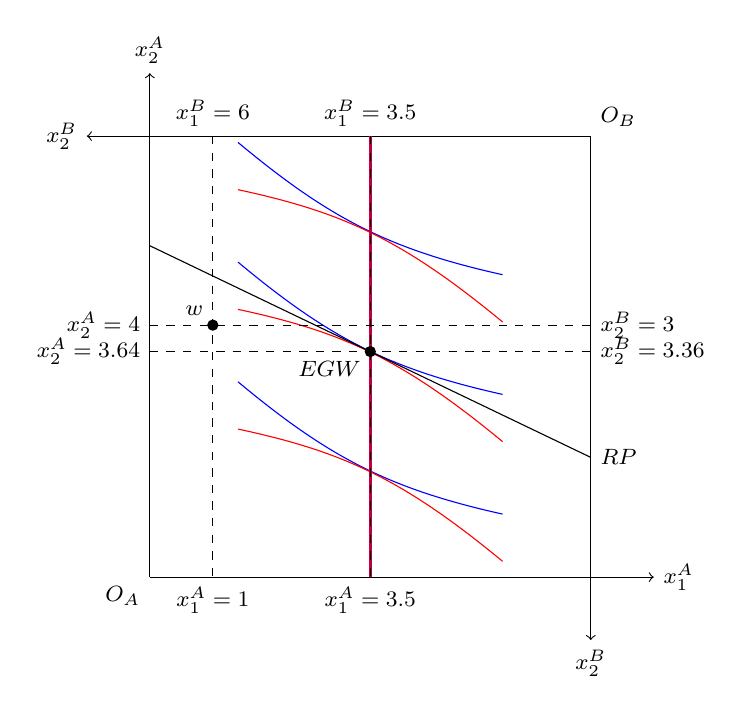
\begin{tikzpicture}[scale=0.8]
			% Formato de CAJA
				\draw[->] (0,0) node[align=center, below left] {\footnotesize $O_A$} -- (0,8) node[align=center, above] {\footnotesize $x_{2}^{A}$};
				\draw[->] (0,0) -- (8,0) node[align=center, right] {\footnotesize $x_{1}^{A}$};
				
				\draw[->] (7,7) node[align=center, above right] {\footnotesize $O_B$} -- (-1,7) node[align=center, left] {\footnotesize $x_{2}^{B}$};
				\draw[->] (7,7) -- (7,-1) node[align=center, below] {\footnotesize $x_{2}^{B}$};
			
			% Curvas de indiferencia
				\draw [blue] (1.4,6.9) .. controls (2.84,5.7) and (3.8,5.2) .. (5.6,4.8);
				\draw [red] (1.4,6.15) .. controls (3.03,5.8) and (3.99,5.38) .. (5.6,4.05);
				
				\draw [blue] (1.4,5) .. controls (2.84,3.8) and (3.8,3.3) .. (5.6,2.9);
				\draw [red] (1.4,4.25) .. controls (3.03,3.9) and (3.99,3.48) .. (5.6,2.15);
				
				\draw [blue] (1.4,3.1) .. controls (2.84,1.9) and (3.8,1.4) .. (5.6,1);
				\draw [red] (1.4,2.35) .. controls (3.03,2) and (3.99,1.58) .. (5.6,0.25);
			
			% Curvas de contrato
				\draw [purple, very thick] (3.5,0) -- (3.5,7);
			
			% Intersección
				\draw[dashed] (1,7) node[above] {\footnotesize $x_{1}^{B}=6$} -- (1,0) node[below] {\footnotesize $x_{1}^{A}=1$};
				\draw[dashed] (0,4) node[left] {\footnotesize $x_{2}^{A}=4$} -- (7,4)node[right] {\footnotesize $x_{2}^{B}=3$};
			
			% Punto
				\draw[black, fill=black] (1,4) circle[radius=0.08] node[align=center, above left] {\footnotesize $w$};
				\draw[black, fill=black] (3.5,3.58) circle[radius=0.08] node[align=center, below left] {\footnotesize $EGW$};
			
			% Recta presupuestaria
				\draw (0,5.26) -- (7,1.9) node[right] {\footnotesize $RP$};
			
			% Intersección
				\draw[dashed] (3.5,7) node[above] {\footnotesize $x_{1}^{B}=3.5$} -- (3.5,0) node[below] {\footnotesize $x_{1}^{A}=3.5$};
				\draw[dashed] (0,3.58) node[left] {\footnotesize $x_{2}^{A}=3.64$} -- (7,3.58)node[right] {\footnotesize $x_{2}^{B}=3.36$};
		\end{tikzpicture}
	\end{center}